\documentclass[aspectratio=169]{beamer}
%\documentclass[xcolor=pst,dvips,epic,eepic]{beamer}

\usepackage[utf8]{inputenc}
\usetheme{Singapore}
\usepackage{xcolor}
\setbeamertemplate{footline}[frame number]

%\usepackage{pgf,pgfarrows,pgfnodes,pgfautomata,pgfheaps,pgfshade}
%\usepackage[pst]{xcolor}
%\usepackage{xxcolor}
\input{../sty/macros}

%\usepackage[frenchb]{babel}
\usepackage{amsmath,amssymb,amsthm}

\usepackage{tikz}
\usetikzlibrary{arrows.meta,decorations.pathreplacing}

\newtheorem{theo}{Theorem}


\usepackage{times}

\setbeamercovered{dynamic}

\def\bomega{\boldsymbol\omega}

\newcommand{\WS}{\mathrm{WS}}
\newcommand{\RP}{\mathrm{RP}}
\newcommand{\EV}{\mathrm{EV}}
\newcommand{\EEV}{\mathrm{EEV}}
\newcommand{\EVPI}{\mathrm{EVPI}}
\newcommand{\VSS}{\mathrm{VSS}}

\author[Fabian Bastin]{Fabian Bastin \\ \texorpdfstring{\url{fabian.bastin@umontreal.ca}}{fabian.bastin@umontreal.ca} \\ Université de Montréal -- CIRRELT -- IVADO}
\date{}
\title[Two-stage SP]{Stochastic optimization\\Two-stage stochastic programming with recourse}

% TODO: the characterisation of K_2 as a polyhedron is still missing. See Birge & Louveaux, Chapter 2.

\begin{document}

\frame{\titlepage}

\begin{frame}
	\frametitle{Formalization}
	
	Uncertainty: representation by means of {\red random elements}.
	The realizations are denoted by $\omega$, and they are drawn from the sample space $\Omega$.
	
	\mbox{}
	
	An {\red event} $A$ is a subset of $\Omega$; the collection of events is denoted by $\mathcal{A}$.
	The event $A \in \mathcal{A}$ occurs if the outcome of the experiment is an element of $A$.
	
\end{frame}

\begin{frame}
	\frametitle{A random linear program}
	\small
	
	Consider the linear program (LP), parametrized by the random vector (r.v.) $\bsxi: \Omega \rightarrow \RR^r$:
	\begin{align*}
		\min_x\ & c^T x \\
		\mbox{s.t. } & Ax = b \\
		& T(\bsxi)x = h(\bsxi) \\
		& x \in X,
	\end{align*}
	with $X = \lbrace x \in \RR^n | l \leq x \leq u \rbrace$. Example:
	\begin{align*}
		\min_x\ & x_1+x_2\\
		\mbox{s.t. } & \bsxi_1x_1 + x_2 \geq 7 \\
		& \bsxi_2x_1 + x_2 \geq 4 \\
		& x_1, x_2 \geq 0,
	\end{align*}
	where $\bsxi_1 \sim U[1,4]$, $\bsxi_2 \sim U[1/3,1]$.
	Slack variables bring the two inequalities back to the equality form above, with $X = \RR^2_+$.
\end{frame}

\begin{frame}
\frametitle{The randomness, seen in the decision space}

Each realization tilts the two constraints: the frontier of the feasible set, and with it the best $x$, moves.

\begin{center}
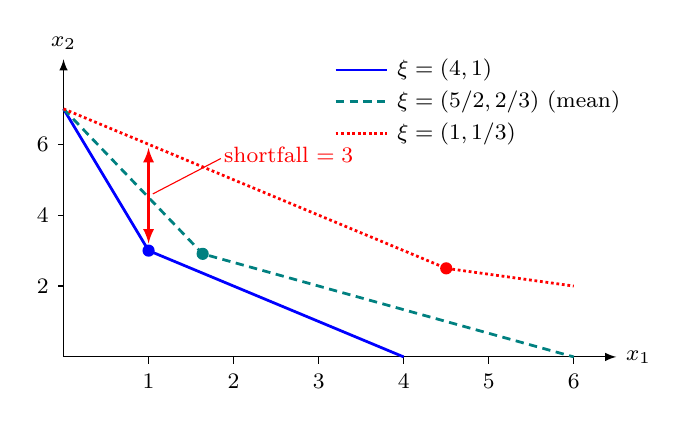
\begin{tikzpicture}[x=1.08cm,y=0.45cm,>=latex,font=\footnotesize]
  \draw[->] (0,0) -- (6.5,0) node[right]{$x_1$};
  \draw[->] (0,0) -- (0,8.4) node[above]{$x_2$};
  \foreach \i in {1,...,6} \draw (\i,0) -- (\i,-0.2) node[below]{$\i$};
  \foreach \j in {2,4,6} \draw (0,\j) -- (-0.06,\j) node[left]{$\j$};
  % frontier of the feasible set (the two binding constraints), per realization
  \draw[blue,line width=1pt]                (0,7) -- (1,3) -- (4,0);
  \draw[teal,line width=1pt,densely dashed] (0,7) -- (1.636,2.909) -- (6,0);
  \draw[red,line width=1pt,densely dotted]  (0,7) -- (4.5,2.5) -- (6,2);
  % optimal vertex for each realization
  \fill[blue] (1,3) circle (2.2pt);
  \fill[teal] (1.636,2.909) circle (2.2pt);
  \fill[red]  (4.5,2.5) circle (2.2pt);
  % the blue optimum is infeasible under the red realization
  \draw[<->,red,thick] (1,3.2) -- (1,5.9);
  \draw[red,thin] (1.05,4.6) -- (1.85,5.6);
  \node[red,right,inner sep=1pt] at (1.85,5.7) {shortfall $=3$};
  % legend
  \draw[blue,line width=1pt]                (3.2,8.1)--(3.8,8.1) node[right,black]{$\xi=(4,1)$};
  \draw[teal,line width=1pt,densely dashed] (3.2,7.2)--(3.8,7.2) node[right,black]{$\xi=(5/2,2/3)$ (mean)};
  \draw[red,line width=1pt,densely dotted]  (3.2,6.3)--(3.8,6.3) node[right,black]{$\xi=(1,1/3)$};
\end{tikzpicture}
\end{center}

The three dots are the three optimal $x$: the one chosen for $\xi=(4,1)$ misses the first constraint by 3 units when $\xi=(1,1/3)$ occurs.

\end{frame}


\begin{frame}
	\frametitle{What to do?}
	
	\begin{itemize}
		\item
		How to solve this problem?
		\item
		What is the {\sl meaning} of solving this problem?
		\item
		Can we decide on $x$ {\sl after} having observed the realization of the r.v. $\bsxi$?\\
		We then talk of a {\red wait-and-see} approach.
		The problem is then easier to solve (we have here a simple linear program).
		\item
		But this approach is rarely appropriate!!! It usually fails to model the
		real behaviour of the decision process: we have to decide on $x$
		{\red before} we know the realizations of $\bsxi$.
		%		\item
		%It the example, we have to decide what to do before we know the realizations $\omega_1$, $\omega_2$.
		\item
		Three suggestions:
		\begin{enumerate}
			\item
			try to estimate, predict, the uncertainty;
			\item
			chance constraints;
			\item
			penalties on deviations.
		\end{enumerate}
	\end{itemize}
	
\end{frame}

\begin{frame}
\frametitle{When is the decision taken?}

\begin{center}
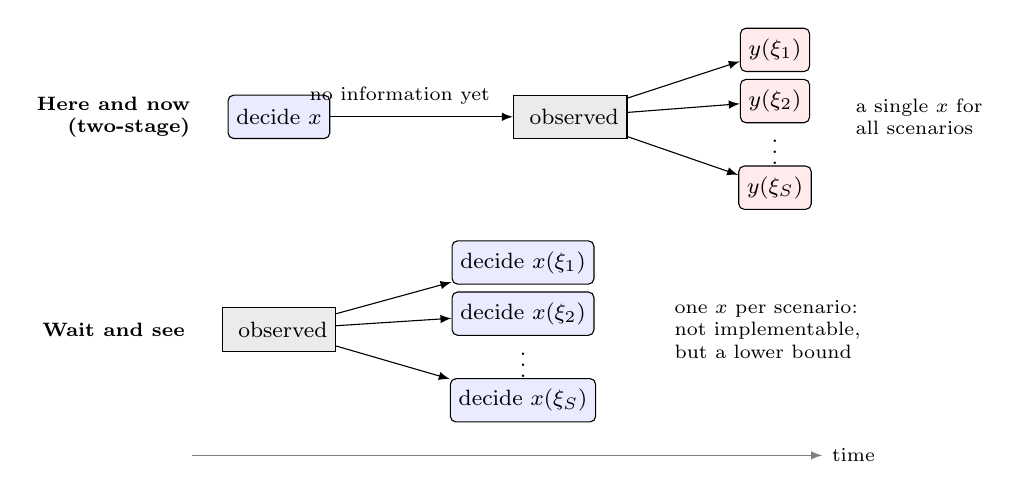
\begin{tikzpicture}[x=1cm,y=1cm,>=latex,font=\footnotesize,
    dec/.style={draw,rounded corners=2pt,fill=blue!8,inner sep=3pt,minimum height=5.5mm},
    rec/.style={draw,rounded corners=2pt,fill=red!8,inner sep=3pt,minimum height=5.5mm},
    ev/.style={draw,fill=black!8,inner sep=3pt,minimum height=5.5mm}]
  % --- here and now
  \node[align=right,font=\scriptsize\bfseries] at (-1.4,0) {Here and now\\(two-stage)};
  \node[dec] (x)  at (0.7,0)    {decide $x$};
  \node[ev]  (o)  at (4.4,0)    {$\bsxi$ observed};
  \node[rec] (y1) at (7.0,0.85) {$y(\xi_1)$};
  \node[rec] (y2) at (7.0,0.2)  {$y(\xi_2)$};
  \node               at (7.0,-0.35) {$\vdots$};
  \node[rec] (yS) at (7.0,-0.9) {$y(\xi_S)$};
  \draw[->] (x) -- node[pos=0.38,above=1pt,font=\scriptsize]{no information yet} (o);
  \draw[->] (o) -- (y1);  \draw[->] (o) -- (y2);  \draw[->] (o) -- (yS);
  \node[right,font=\scriptsize,align=left] at (7.9,0) {a single $x$ for\\all scenarios};
  % --- wait and see
  \node[align=right,font=\scriptsize\bfseries] at (-1.4,-2.7) {Wait and see};
  \node[ev]  (o2) at (0.7,-2.7)   {$\bsxi$ observed};
  \node[dec] (x1) at (3.8,-1.85)  {decide $x(\xi_1)$};
  \node[dec] (x2) at (3.8,-2.5)   {decide $x(\xi_2)$};
  \node                at (3.8,-3.05) {$\vdots$};
  \node[dec] (xS) at (3.8,-3.6)   {decide $x(\xi_S)$};
  \draw[->] (o2) -- (x1);  \draw[->] (o2) -- (x2);  \draw[->] (o2) -- (xS);
  \node[right,font=\scriptsize,align=left] at (5.6,-2.7) {one $x$ per scenario:\\not implementable,\\but a lower bound};
  \draw[->,gray] (-0.4,-4.3) -- (7.6,-4.3) node[right,black,font=\scriptsize]{time};
\end{tikzpicture}
\end{center}

\end{frame}


\begin{frame}
	\frametitle{Remove the randomness?}
	
	A popular approach consists in looking for reasonable values for $\bsxi_1$ and $\bsxi_2$.
	How?
	
	\mbox{}
	
	Propositions:
	\begin{itemize}
		\item unbiased: choose the mean values for each random variable;
		\item pessimistic: choose the worst-case values for $\bsxi$;
		\item optimistic: choose the best-case values for $\bsxi$.
	\end{itemize}
	
	Each approach will deliver a different optimal solution!
	
\end{frame}

\begin{frame}
	\frametitle{Penalization of violations}
	
	Again, we have to deal with decision problems where the decision $x$ has to be taken before we know the realization of $\bsxi$
	
	In the simplest case, we can simply penalize the constraints deviations by vectors of penalty coefficients $q_+$ and $q_-$.
	\begin{align*}
	\min\ & c^Tx+q^T_+s(\bsxi)+q^T_-t(\bsxi) \\
	\mbox{s.t. } & Ax = b, \\
	& T(\bsxi)x + s(\bsxi)-t(\bsxi) = h(\bsxi), \\
	& x \in X, \quad s(\bsxi) \geq 0, \quad t(\bsxi) \geq 0.
	\end{align*}
	
	\mbox{}
	
	But it is still not possible to solve the problem!
	
\end{frame}

\begin{frame}
	\frametitle{The new optimization problem}
	
	A reasonable, and solvable, problem is then
	\begin{align*}
	\min\ & c^Tx+\EE_{\bsxi}[q^T_+s(\bsxi)+q^T_-t(\bsxi)] \\
	\mbox{s.t. } & Ax = b, \\
	& T(\xi)x + s(\xi)-t(\xi) = h(\xi),\ \text{ for a.e. } \xi \\
	& x \in X, \quad s(\xi) \geq 0,\ t(\xi) \geq 0,\ \text{ for a.e. } \xi,
	\end{align*}
where {\it a.e.} stands for ``almost every''.
	\begin{itemize}
		\item
		In general, we can react in a correct (and maybe optimal) way: we have a recourse to ``correct'' the first decision once the uncertainty is removed.
		\item
		An LP recourse structure is provided by 3 elements:
		\begin{itemize}
			\item
			a set $Y \subset \RR^p$ that describes the feasible set of recourse actions, for instance $Y = \lbrace y \in \RR^p \,|\, y \geq 0 \rbrace$;
			\item
			$q$: a vector of recourse costs;
			\item
			$W \in \RR^{m \times p}$: {\blue recourse matrix}.
		\end{itemize}
	\end{itemize}
	
\end{frame}

\begin{frame}
	\frametitle{Recourse formulation}
	
	More generally, consider the following program:
	\begin{align*}
	\min\ & c^Tx+\EE_{\bsxi}[q(\bsxi)^Ty(\bsxi)] \\
	\mbox{s.t. } & Ax = b, \\
	& T(\xi)x + Wy(\xi) = h(\xi),\ \text{ for a.e. } \xi \\
	& x \in X, \\
	& y(\xi) \in Y,\ \text{ for a.e. } \xi.
	\end{align*}
	
	We could have $W$ varying with the realization $\xi$.
	If $W$ is unique, as in the previous formulation, we speak of {\red fixed recourse}: the recourse does not change with the scenario.\\
	But how to decide on $y$?
	
\end{frame}

\begin{frame}
	\frametitle{The two-stage linear stochastic problem (SP)}
	
	We can also rewrite the stochastic programming problem with recourse in terms of $x$ only:
	\[
	\min_{x \in X} \lbrace c^T x + \mathcal{Q}(x) \ |\  Ax = b \rbrace.
	\]
	It is a (nonlinear) mathematical programming problem in $\RR^n$.
	
	The properties of $\mathcal{Q}(x)$ influence the solution techniques.
	
	\mbox{}
	
	Is $\mathcal{Q}(x)$
	\begin{itemize}
		\item
		linear?
		\item
		convex?
		\item
		continuous?
		\item
		differentiable?
	\end{itemize}
	
\end{frame}

\begin{frame}
	\frametitle{Expression in terms of $y$'s}
	
	\begin{align*}
	\min_{x,\ y(\bsxi)}\ & \EE_{\bsxi} [ c^T x + q(\bsxi)^T y(\bsxi) ] \\
	\mbox{s.t. } & Ax = b & \mbox{\textcolor{blue}{first-stage constraints}} \\
	& T(\xi)x + Wy(\xi) = h(\xi),\ \text{ for a.e. } \xi &
	\mbox{\textcolor{blue}{second-stage constraints}} \\
	& x \in X,\ y(\xi) \in Y\ \text{ for a.e. } \xi.
	\end{align*}
	
	\mbox{}
	
	Consider the (discrete) case where $\Omega = \lbrace \omega_1,\
	\omega_2,\ldots,\omega_S \rbrace$, with support $\Xi = \bsxi(\Omega) \subseteq \RR^r$.
	\begin{align*}
	P[\lbrace \omega_s \rbrace] & = p_s,\ s = 1, 2,\ldots, S \\
	q_s & = q(\xi(\omega_s)),\ T_s = T (\xi(\omega_s)),\ h_s = h(\xi(\omega_s))
	\end{align*}
	
\end{frame}

\begin{frame}
	\frametitle{Deterministic equivalent}
	
	Develop along the $S$ scenarios.
	\begin{align*}
	\min_{x, y_1, \ldots, y_S}\ & c^T x + p_1 q_1^T y_1 + p_2 q_2^T y_2 + \ldots
	+ p_S q_S^Ty_S \\
	\mbox{s.t. } & \\
	& \begin{matrix} Ax & & & & & = b\\
	T_1 x & + W y_1 & & & & = h_1 \\
	T_2 x & & + W y_2 & & & = h_2 \\
	\vdots & & & \ddots & \\
	T_S x & & & & + W y_S & = h_S
	\end{matrix} \\
	& x \in X,\ y_1 \in Y,\ y_2 \in Y,\ldots, y_S \in Y.
	\end{align*}
	
\end{frame}

\begin{frame}
	\frametitle{Deterministic equivalent (cont'd)}
	
	\begin{itemize}
		\item
		$y_s = y(\xi(\omega_s))$: recourse action to take if the scenario
		$s$ occurs.
		\item
		\textcolor{blue}{Advantage}: linear program.
		\item
		\textcolor{blue}{Drawback}: linear program of (very) large dimension:
		\begin{itemize}
			\item
			$n+pS$ variables;
			\item
			$m_1+mS$ constraints, with $A \in \RR^{m_1 \times n}$ and
			$W \in \RR^{m \times p}$.
		\end{itemize}
		\item
		\textcolor{blue}{Advantage}: the linear program matrix has a special structure (stairway shape).\\
		Can we exploit it?
	\end{itemize}
	
\end{frame}

\begin{frame}
\frametitle{The staircase structure}

\begin{center}
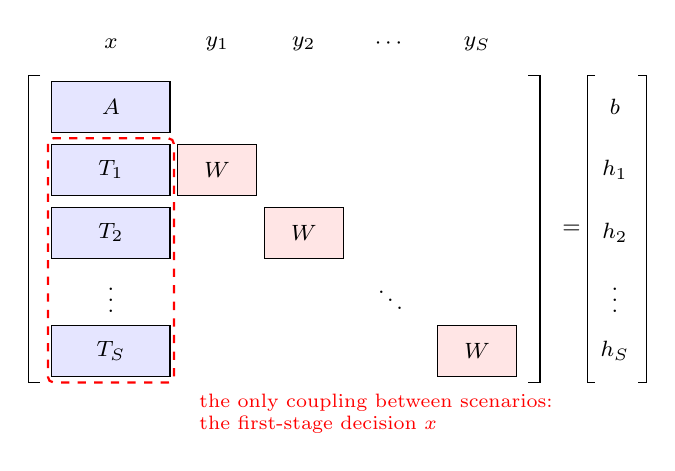
\begin{tikzpicture}[x=1cm,y=1cm,font=\footnotesize,
   blk/.style={draw,minimum height=6.5mm,inner sep=1pt}]
  % variable names
  \node at (0.75,0.45) {$x$};
  \node at (2.1,0.45) {$y_1$};  \node at (3.2,0.45) {$y_2$};
  \node at (4.3,0.45) {$\cdots$}; \node at (5.4,0.45) {$y_S$};
  % blocks
  \node[blk,minimum width=1.5cm,fill=blue!10] at (0.75,-0.35) {$A$};
  \node[blk,minimum width=1.5cm,fill=blue!10] at (0.75,-1.15) {$T_1$};
  \node[blk,minimum width=1.5cm,fill=blue!10] at (0.75,-1.95) {$T_2$};
  \node                                        at (0.75,-2.7)  {$\vdots$};
  \node[blk,minimum width=1.5cm,fill=blue!10] at (0.75,-3.45) {$T_S$};
  \node[blk,minimum width=1cm,fill=red!10]    at (2.1,-1.15) {$W$};
  \node[blk,minimum width=1cm,fill=red!10]    at (3.2,-1.95) {$W$};
  \node                                        at (4.3,-2.7)  {$\ddots$};
  \node[blk,minimum width=1cm,fill=red!10]    at (5.4,-3.45) {$W$};
  % brackets
  \draw (-0.15,0.05) -- (-0.3,0.05) -- (-0.3,-3.85) -- (-0.15,-3.85);
  \draw (6.05,0.05) -- (6.2,0.05) -- (6.2,-3.85) -- (6.05,-3.85);
  % right-hand side
  \node at (6.6,-1.9) {$=$};
  \draw (6.9,0.05) -- (6.8,0.05) -- (6.8,-3.85) -- (6.9,-3.85);
  \node at (7.15,-0.35) {$b$};   \node at (7.15,-1.15) {$h_1$};
  \node at (7.15,-1.95) {$h_2$}; \node at (7.15,-2.7)  {$\vdots$};
  \node at (7.15,-3.45) {$h_S$};
  \draw (7.45,0.05) -- (7.55,0.05) -- (7.55,-3.85) -- (7.45,-3.85);
  % the coupling column
  \draw[red,thick,dashed,rounded corners=2pt] (-0.05,-0.75) rectangle (1.55,-3.85);
  \node[red,right,align=left,font=\scriptsize] at (1.75,-4.25)
     {the only coupling between scenarios:\\the first-stage decision $x$};
\end{tikzpicture}
\end{center}

Delete that first column and the problem falls apart into $S$ independent small programs: this is what the decomposition methods of the next chapter exploit.

\end{frame}


\begin{frame}
	\frametitle{Large scale,\ldots and?}
	
	Assume that we have $r$ random variables ($\Xi \subseteq
	\RR^r$).
	\begin{itemize}
		\item
		Consider the following problem (source: Linderoth).
		A Telecom company wants to expand its network in order to meet an unknown (random) demand.
		\item
		There are 86 unknown demands.
		Each demand is independent and takes a value in a set of 7 values.
		Consequently
		\[
		S = |\Omega| = 7^{86} \approx 4.77\times10^{72}.
		\]
		For comparison, the observable universe is estimated to hold some
		$10^{80}$ atoms.
		\item
		It can be even worse\ldots\\
		If $\Omega$ is not finite, but holds an infinite number of elements?
		It is especially true with continuous random variables.
		Our ``deterministic equivalent'' would have an infinite number of variables and constraints!
		\item
		We can solve an approximate problem, obtained by sampling over the random vector.
	\end{itemize}
\end{frame}

\begin{frame}
	\frametitle{An example (cont'd)}
	
	Consider again our toy problem
	\begin{align*}
	\min_x\ & x_1+x_2\\
	\mbox{s.t. } & \bsxi_1x_1 + x_2 \geq 7 \\
	& \bsxi_2x_1 + x_2 \geq 4 \\
	& x_1, x_2 \geq 0,
	\end{align*}
	where $\bsxi_1 \sim U[1,4]$, $\bsxi_2 \sim U[1/3,1]$.
	
	\mbox{}
	
	How to build the deterministic equivalent?
	
\end{frame}

\begin{frame}
	\frametitle{Example: recourse formulation}
	
	Assume for now that $\Omega$ is finite, with $S$ scenarios.
	\begin{align*}
	\min_{x,\, y}\ & x_1+x_2 + \sum_{s = 1}^{S} p_s q (y_{1s} + y_{2s})\\
	\mbox{s.t. } & \xi_{1s}x_1 + x_2 + y_{1s} \geq 7, & s = 1,\ldots,S \\
	& \xi_{2s}x_1 + x_2 + y_{2s} \geq 4, & s = 1,\ldots,S \\
	& x_1, x_2 \geq 0,\\
	& y_{1s}, y_{2s} \geq 0, & s = 1,\ldots,S.
	\end{align*}
	
	A difficulty is therefore to decide how to construct the deterministic equivalent.
	How to choose $q$?
	
	\mbox{}
	
	How to construct the scenarios?
	We can proceed with Monte Carlo sampling, with $p_s = 1/S$, $\forall s$.
	We will explore this approach in more details later.
	
\end{frame}

\begin{frame}
	\frametitle{Example: recourse formulation (cont'd)}
	
	More generally, we can build the program
	\begin{align*}
	\min_x\ & x_1+x_2 + \EE_{\bsxi}[Q(x,\bsxi)] \\
	\mbox{s.t. } & x_1, x_2 \geq 0,
	\end{align*}
	and
	\begin{align*}
	Q(x, \xi) = \min_y\ & q_1y_1 + q_2y_2 \qquad (q_1 = q_2 = q \text{ above}) \\
	\mbox{s.t. } & \xi_1 x_1 + x_2 + y_1 \geq 7, \\
	& \xi_2 x_1 + x_2 + y_2 \geq 4, \\
	& y_1, y_2 \geq 0.
	\end{align*}
	
\end{frame}

\begin{frame}
\frametitle{Two-stage linear programming problem, fixed recourse}

We go a bit further by considering the problem
\[
\min c^Tx + \EE_{\bsxi}[q(\bsxi)^Ty(\bsxi)]
\]
subject to the constraints
\begin{align*}
Ax &= b, \\
T(\xi)x + Wy(\xi) &= h(\xi) \qquad \text{for a.e. } \xi \in \Xi, \\
x & \in X, \\
y(\xi) & \in Y \qquad \text{for a.e. } \xi \in \Xi,
\end{align*}
where $\bsxi$ is a random vector defined on the probability space 
$(\Omega, \mathcal{F}, P)$, and $\Xi$ is the support of $\bsxi$.

\end{frame}

\begin{frame}
\frametitle{Reformulation(s)}

The problem becomes
\[
\min_{x \in X \,|\, Ax = b} \left\lbrace c^Tx + \EE_{\bsxi} \left[ \min_{y \in Y} \left\lbrace q(\bsxi)^Ty \ |\ Wy = h(\bsxi) - T(\bsxi)x \right\rbrace \right] \right\rbrace,
\]
or
\[
\min_{x \in X \,|\, Ax = b} c^Tx + \EE_{\bsxi} [ Q(x,\bsxi)], 
\]
with
\[
Q(x, \xi) = \min_{y \in Y} \left\lbrace q(\xi)^Ty: Wy = h(\xi) - T(\xi)x \right\rbrace.
\]

\smallskip

{\red Second-stage function}, or {\red recourse function}, $v: \Xi \times \RR^m \rightarrow \overline{\RR} = \RR \cup \lbrace \pm\infty \rbrace$:
\[
v(\xi, z) \overset{\mathrm{def}}{=} \min_{y \in Y} \lbrace q(\xi)^Ty \ |\ Wy = z \rbrace.
\]

\smallskip

Given a ``policy'' $x$ and a realization $\xi$, $z$ measures the deviation of the first stage, i.e. $z = h(\xi) - T(\xi)x$, $v(\xi, z)$ is the minimum cost to ``correct'' the decision. % in order to satisfy the constraints again.

\end{frame}

\begin{frame}
\frametitle{Recourse function}

{\red Expected recourse function}:
%, or the function of minimum expected recourse, $\mathcal{Q}: \RR^n \rightarrow \RR$, for any policy $x \in \RR^n$:
\[
\mathcal{Q}(x) \overset{\mathrm{def}}{=} \EE_{\bsxi}[Q(x,\bsxi)],
\]
%describes the recourse cost expectation,
with
\[
Q(x, \xi) = v(\xi, h(\xi)-T(\xi)x).
\]

\mbox{}

%With these definitions, 
The problem can now be rewritten as:
\[
\min_{x \in X} c^Tx + \mathcal{Q}(x) \mbox{ such that } Ax = b.
\]
It is a nonlinear program over $\RR^n$. Properties?
\end{frame}

\begin{frame}
\frametitle{Formulations summary}

Set $X = \RR^n_+$.
\[
\min_{x \in \RR^n_+ \,|\, Ax = b} \left\lbrace c^Tx + \EE_{\bsxi} \left[ \min_{y \in \RR^p_+} \lbrace q(\bsxi)^Ty \ |\ Wy = h(\bsxi) - T(\bsxi)x \rbrace \right] \right\rbrace 
\]
\[
\min_{x \in \RR^n_+ \,|\, Ax = b} \left\lbrace c^Tx + \EE_{\bsxi}
  \left[  v(\bsxi, h(\bsxi)-T(\bsxi)x) \right] \right\rbrace 
\]
\[
\min_{x \in \RR^n_+ \,|\, Ax = b} \left\lbrace c^Tx + \EE_{\bsxi} \left[ Q(x,\bsxi) \right] \right\rbrace 
\]
\[
\min_{x \in \RR^n_+} \left\lbrace c^Tx + \mathcal{Q}(x)
  \ |\ Ax = b \right\rbrace 
\]

\end{frame}

\begin{frame}
\frametitle{Notations}

\begin{itemize}
\item
{\red First-stage feasible set}:
\[
K_1 = \lbrace x \in \RR^n_+ \ |\ Ax = b \rbrace.
\]
\item
{\red Second-stage strong feasible set}:
\[
K_2^s = \lbrace x \ |\ \mathcal{Q}(x) < \infty \rbrace.
\]
\end{itemize}

\mbox{}

Therefore we can rewrite the problem as
\[
\min_x \lbrace c^Tx + \mathcal{Q}(x) \ |\ x \in K_1 \cap K_2^s \rbrace.
\]

\end{frame}

\begin{frame}
\frametitle{Weak feasible set}

See Walkup, D. W. and Wets, R. J.-B., {\it Stochastic programs with recourse}, SIAM Journal on Applied Mathematics, 15(5):1299--1314, 1967.

\mbox{}

{\red Positive hull} (or conical hull)
$$
\text{pos}W = \lbrace z \,|\, z = Wy,\ y \in \RR^p_+ \rbrace
$$
(positive hulls and Farkas' lemma are recalled in the linear programming background notes)

\mbox{}

{\red Weak second-stage feasible set}
\begin{align*}
K_2 &= \lbrace x \in \RR^n \,|\, Q(x,\xi) < +\infty \text{ a.s.} \rbrace \\
&= \lbrace x \in \RR^n \,|\, (h(\xi) - T(\xi)x) \in \text{pos} W \text{ a.s.} \rbrace
\end{align*}

\end{frame}

\begin{frame}
\frametitle{pos$\,W$, graphically}

$\mathrm{pos}\,W$ is the cone spanned by the columns of $W$ with non-negative weights: the set of right-hand sides $z$ that the recourse can absorb.

\begin{center}
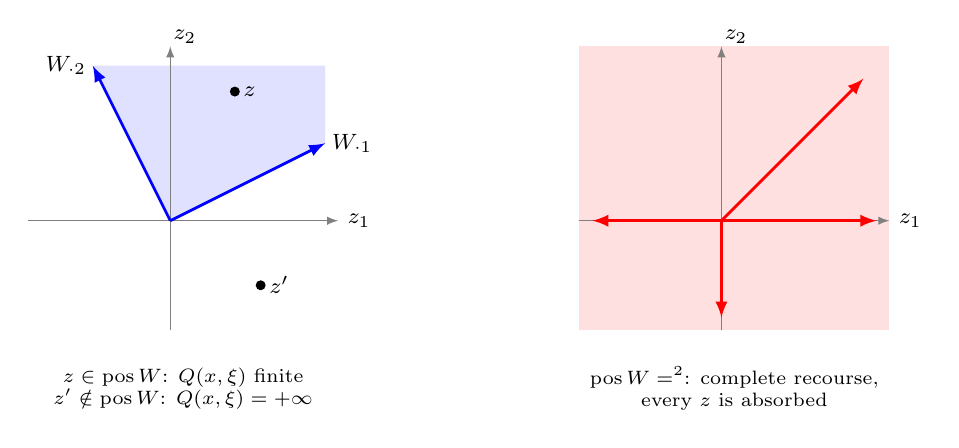
\begin{tikzpicture}[x=0.82cm,y=0.82cm,>=latex,font=\footnotesize]
  % ---------------- panel A: pointed cone
  \fill[blue!12] (0,0) -- (2.4,1.2) -- (2.4,2.4) -- (-1.2,2.4) -- cycle;
  \draw[->,gray] (-2.2,0) -- (2.6,0) node[right,black]{$z_1$};
  \draw[->,gray] (0,-1.7) -- (0,2.7) node[above right,black,inner sep=1pt]{$z_2$};
  \draw[->,blue,line width=1pt] (0,0) -- (2.4,1.2) node[right,black,inner sep=2pt]{$W_{\cdot 1}$};
  \draw[->,blue,line width=1pt] (0,0) -- (-1.2,2.4) node[left,black,inner sep=2pt]{$W_{\cdot 2}$};
  \fill (1,2) circle (1.8pt) node[right,inner sep=3pt]{$z$};
  \fill (1.4,-1.0) circle (1.8pt) node[right,inner sep=3pt]{$z'$};
  \node[align=center,font=\scriptsize] at (0.2,-2.6)
     {$z \in \mathrm{pos}\,W$: $Q(x,\xi)$ finite\\
      $z' \notin \mathrm{pos}\,W$: $Q(x,\xi) = +\infty$};
  % ---------------- panel B: whole plane
  \begin{scope}[xshift=7cm]
    \fill[red!12] (-2.2,-1.7) rectangle (2.6,2.7);
    \draw[->,gray] (-2.2,0) -- (2.6,0) node[right,black]{$z_1$};
    \draw[->,gray] (0,-1.7) -- (0,2.7) node[above right,black,inner sep=1pt]{$z_2$};
    \draw[->,red,line width=1pt] (0,0) -- (2.2,2.2);
    \draw[->,red,line width=1pt] (0,0) -- (2.4,0);
    \draw[->,red,line width=1pt] (0,0) -- (-2.0,0);
    \draw[->,red,line width=1pt] (0,0) -- (0,-1.5);
    \node[align=center,font=\scriptsize] at (0.2,-2.6)
      {$\mathrm{pos}\,W = \RR^2$: {\red complete recourse},\\every $z$ is absorbed};
  \end{scope}
\end{tikzpicture}
\end{center}

\end{frame}


\begin{frame}
\frametitle{Relatively complete recourse}

A problem is said to have a {\red relatively complete recourse} if $K_1
\subseteq K_2$.

\mbox{}

{\blue Advantage}: the second-stage problem is feasible $\forall x$ feasible in the first stage, almost surely (i.e. with probability equal to 1).
%Reminder: almost surely, or with probability one. An event $A$ is said to occur almost surely if $P[A] = 1$.



\mbox{}

{\blue Issue}: $K_2^s \subseteq K_2$. We would like $K_2^s = K_2$.

\end{frame}

\begin{frame}
\frametitle{Complete recourse}
	
\begin{itemize}
	\item 
	The relatively complete recourse is very useful in practice and on a theoretical point of view, but it can be difficult to identify.
%	\item 
%	A particular case of relatively complete recourse can however often be identified from the structure of $W$.
\item
	{\red Complete recourse}: $\text{pos}W = \RR^m$, i.e. $\forall z \in \RR^m$, $\exists y \in \RR^p_+$ such that $Wy = z$.
	\item
	Complete recourse $\Rightarrow$ relatively complete recourse, as 
$\forall x$, $T(\xi)$, $h(\xi)$, $Q(x,\xi) < \infty$ with $z = h(\xi)-T(\xi)x$.
\end{itemize}

\end{frame}

\begin{frame}
\frametitle{$K_1$, $K_2$, and the two notions of completeness}

\begin{center}
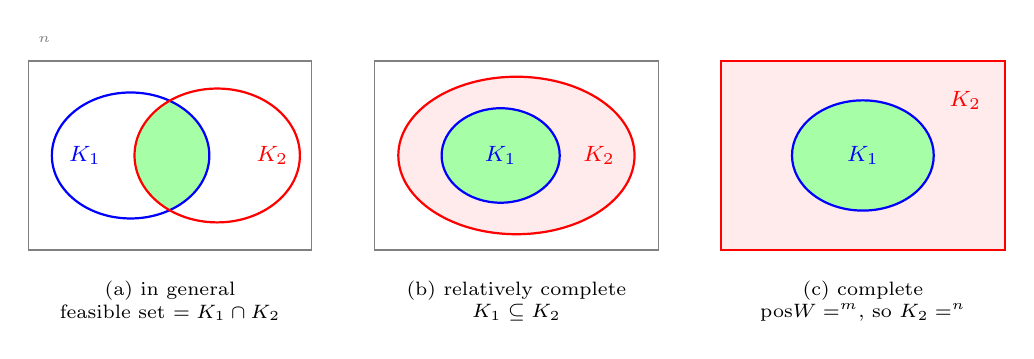
\begin{tikzpicture}[x=1cm,y=1cm,font=\footnotesize]
  % (a)
  \draw[gray] (0,0) rectangle (3.6,2.4);
  \node[gray,above right,font=\scriptsize] at (0,2.4) {$\RR^n$};
  \begin{scope}
    \clip (1.3,1.2) ellipse (1.0 and 0.8);
    \fill[green!35] (2.4,1.2) ellipse (1.05 and 0.85);
  \end{scope}
  \draw[blue,thick] (1.3,1.2) ellipse (1.0 and 0.8);
  \draw[red,thick]  (2.4,1.2) ellipse (1.05 and 0.85);
  \node[blue] at (0.72,1.2) {$K_1$};  \node[red] at (3.1,1.2) {$K_2$};
  \node[align=center,font=\scriptsize] at (1.8,-0.65) {(a) in general\\feasible set $=K_1\cap K_2$};
  % (b)
  \begin{scope}[xshift=4.4cm]
    \draw[gray] (0,0) rectangle (3.6,2.4);
    \draw[red,thick,fill=red!8]    (1.8,1.2) ellipse (1.5 and 1.0);
    \draw[blue,thick,fill=green!35] (1.6,1.2) ellipse (0.75 and 0.6);
    \node[blue] at (1.6,1.2) {$K_1$};  \node[red] at (2.85,1.2) {$K_2$};
    \node[align=center,font=\scriptsize] at (1.8,-0.65) {(b) relatively complete\\$K_1 \subseteq K_2$};
  \end{scope}
  % (c)
  \begin{scope}[xshift=8.8cm]
    \draw[red,thick,fill=red!8] (0,0) rectangle (3.6,2.4);
    \draw[blue,thick,fill=green!35] (1.8,1.2) ellipse (0.9 and 0.7);
    \node[blue] at (1.8,1.2) {$K_1$};  \node[red] at (3.1,1.9) {$K_2$};
    \node[align=center,font=\scriptsize] at (1.8,-0.65) {(c) complete\\$\mathrm{pos}W=\RR^m$, so $K_2=\RR^n$};
  \end{scope}
\end{tikzpicture}
\end{center}

\smallskip

Completeness is read off $W$ alone; relative completeness also depends on $A$, $b$ and on the support of $\bsxi$, and is the property that really matters: it is what forbids a first-stage decision to be caught infeasible in the second stage.

\end{frame}


\begin{frame}
\frametitle{$K_2 \ne K_2^s$}

Consider the second-stage problem
\begin{align*}
	\min_y\ & 2y_1+y_2\\
	\mbox{s.t. } & y_1 + y_2 \geq 1 - x_1,\\
	& y_1 \geq \xi - x_1 - x_2,\\
	& y_1, y_2 \geq 0,
\end{align*}
with
$$
P\left[ \bsxi = 2^n \right] = \frac{1}{2^{n+1}},\ n = 0,1,2,\ldots
$$
Note that $P\left[ \bsxi = 2^n \right] \in (0,1),\ n = 0,1,2,\ldots$, $\Xi = \lbrace 2^n,\ n = 0, 1, 2, \ldots \rbrace$, and
$$
\sum_{n=0}^{+\infty} P\left[ \bsxi = 2^n \right] = \sum_{n=0}^{+\infty} 2^{-n-1} = \frac{1}{2} \frac{1}{1-\frac{1}{2}} = 1.
$$

\end{frame}

\begin{frame}
\frametitle{$K_2 \ne K_2^s$ (cont'd)}

Given $x \in \RR^2$, we have
\begin{align*}
\calQ(x) &= \EE_{\bsxi} \left[ \min_{y \geq 0} 2y_1+y_2 \,\bigg|\, y_1 + y_2 \geq 1 - x_1,\ y_1 \geq \bsxi - x_1 - x_2 \right] \\
&\geq \EE_{\bsxi} \left[ \min_{y_1 \geq 0} 2y_1 \,\bigg|\, y_1 \geq \bsxi - x_1 - x_2 \right] \\
& = 2 \EE_{\bsxi} \left[ \max \{ 0, \bsxi - x_1 - x_2 \}\right] \\
& = 2 \sum_{\xi \in \Xi} P[\bsxi = \xi] \max \{ 0, \xi - x_1 - x_2 \} \\
& = 2 \sum_{n = 0}^{+\infty} 2^{-n-1} \max \{ 0, 2^n - x_1 - x_2 \} \\
& = \sum_{n = 0}^{+\infty} 2^{-n} \max \{ 0, 2^n - x_1 - x_2 \} = +\infty
\end{align*}

\end{frame}

\begin{frame}
\frametitle{$K_2 \ne K_2^s$ (cont'd)}

Thus, $K_2^s = \emptyset$.

\mbox{}

The problem, set under standard form, can be rewritten as
\begin{align*}
	\min_{y,u}\ & 2y_1+y_2\\
	\mbox{s.t. } & y_1 + y_2 - u_1 = 1 - x_1,\\
	& y_1 -u_2 = \xi - x_1 - x_2,\\
	& y_1, y_2, u_1, u_2 \geq 0,
\end{align*}
and
$$
W = \begin{pmatrix}
 1 & 1 & -1 & 0 \\ 1 & 0 & 0 & -1
\end{pmatrix}.
$$
$\text{pos} W = ?$

\end{frame}

\begin{frame}
\frametitle{$K_2 \ne K_2^s$ (cont'd)}

Complete recourse if pos$W = \RR^2$, i.e.
$$
\forall z \in \RR^2, \exists y \geq 0, u \geq 0 \text{ s.t. } W\begin{pmatrix} y \\ u \end{pmatrix} = z.
$$
We have that
\begin{align*}
& W\begin{pmatrix} y \\ u \end{pmatrix} = \begin{pmatrix} y_1 + y_2 - u_1 \\ y_1 - u_2 \end{pmatrix} = z \\
\Leftrightarrow &
\begin{cases}
	y_1 + y_2 - u_1 &= z_1, \\ y_1 - u_2 &= z_2.
\end{cases}
\end{align*}
Thus, we can take
$$
\begin{cases}
 y_1 = z_2,\ u_2 = 0, & \text{ if } z_2 \geq 0,\\
 y_1 = 0,\ u_2 = -z_2, & \text{ otherwise}.
\end{cases}
$$

\end{frame}

\begin{frame}
\frametitle{$K_2 \ne K_2^s$ (cont'd)}

Then, writing $y_2 - u_1 = z_1 - y_1$, we take
$$
\begin{cases}
	y_2 = z_1 - y_1,\ u_1 = 0, & \text{ if } z_1 - y_1 \geq 0,\\
	y_2 = 0,\ u_1 = y_1 - z_1, & \text{ otherwise}.
\end{cases}
$$
Thus,
\begin{itemize}
	\item 
	pos$W = \RR^2$, and the recourse is complete,
	\item
	$K_2 = \RR^2$, and the recourse is relatively complete,
	\item
	{\red $K_2 \ne K_2^s$}.
\end{itemize}

\mbox{}

Note that
$$
\EE[\bsxi] = \sum_{n=0}^{+\infty} P\left[ \bsxi = 2^n \right] 2^n = \sum_{n=0}^{+\infty} \frac{2^n}{2^{n+1}} = \sum_{n=0}^{+\infty} \frac{1}{2} = +\infty.
$$

\end{frame}

\begin{frame}
\frametitle{$K_2 \ne K_2^s$ (cont'd)}

$\EE[\bsxi]$ not finite does not necessarily imply that $\calQ(x) = +\infty$. Consider
\begin{align*}
\min_y \ & y_1 - y_2 \\
\text{s.t. } & y_1 \geq \xi, \\
& y_2 \leq \xi, \\
& y_1,\ y_2 \geq 0.
\end{align*}
The optimum is attained at $y_1 = y_2 = \xi$, so $Q(x, \xi) = 0$ for all $\xi$ (and all $x$), and therefore $\calQ(x) = 0$.

\end{frame}

\begin{frame}
\frametitle{$K_2 = K_2^s$}

\begin{theo}
For a stochastic program with fixed recourse, where $\bsxi$ has finite second-order moments,
$$
P\left[ Q(x,\bsxi) < \infty \right] = 1 \Longrightarrow \mathcal{Q}(x) < \infty,
$$
and consequently
$$
K_2 = K_2^s.
$$
\end{theo}

%In other words, we must have that $Q(x,\bsxi)$ is upper bounded almost surely. Proof: technical!

\end{frame}

\begin{frame}
\frametitle{Elementary feasible set}

\begin{itemize}
	\item 
Given a realization $\xi$, the {\red elementary second-stage feasible set} is defined as:
\[
K_2(\xi) = \lbrace x \ |\ Q(x,\xi) < \infty \rbrace.
\]
\item
Define {\red possibility interpretation} of the second-stage feasibility as
\[
K_2^P = \cap_{\xi \in \Xi} K_2(\xi).
\]
\item
Clearly $K_2 = K_2^P$ if $\bsxi$ has a finite support, every scenario having a positive probability.
Is it still the case when $\bsxi$ follows a continuous distribution?
\end{itemize}

\end{frame}

\begin{frame}
\frametitle{Elementary feasible set (cont'd)}

\begin{theo}
For a stochastic program with fixed recourse, where $\bsxi$ has finite second-order moments,
$$K_2 = K_2^s = K_2^P.$$
\end{theo}

With a fixed recourse, $x \in K_2(\xi) \iff h(\xi)-T(\xi)x \in \text{pos}W$, a {\red closed} cone: the set of favourable $\xi$ is then closed, and having probability one forces it to contain the whole support.
The exercise below shows what happens when the recourse is not fixed.

\end{frame}

\begin{frame}
\frametitle{Simple recourse}

A particular case of complete recourse is the {\red simple recourse}, for which we have
\[
W = \begin{pmatrix} I & -I \end{pmatrix},
\]
with $I$ the identity matrix, of order $m$.

\mbox{}

pos$W = \RR^m$: writing
$$
y = \begin{pmatrix}
	y^+ \\ y^-
\end{pmatrix},
$$
where $y \in \RR^{2m}$, $y^+, y^- \in \RR^m$, for $z \in \RR^m$, we can solve
$$
Wy = z,\ y \geq 0,
$$
by choosing $y^+ = \max\{z,0\}$,  $y^- = \max\{-z,0\}$.

\end{frame}

\begin{frame}
\frametitle{Simple recourse (cont'd)}

The second stage program can be read as
\begin{align*}
Q(x,\xi) & = \min_y q^+(\xi)^Ty^+ + q^-(\xi)^Ty^- \\
\mbox{s.t. } & y^+ - y^- = h(\xi)-T(\xi)x,\\
& y^+,\ y^- \geq 0.
\end{align*}
That is, for $q^+(\xi) + q^-(\xi) \geq 0$, at most one of $y_i^+$ and $y_i^-$ is positive at the optimum, so they %(non negatively)
measure the positive and negative parts of the discrepancy $h(\xi)-T(\xi)x$.

\end{frame}

\begin{frame}
\frametitle{Simple recourse, graphically}

With $m = 1$, write $z = h(\xi)-T(\xi)x$ for the discrepancy left by the first stage.

\begin{center}
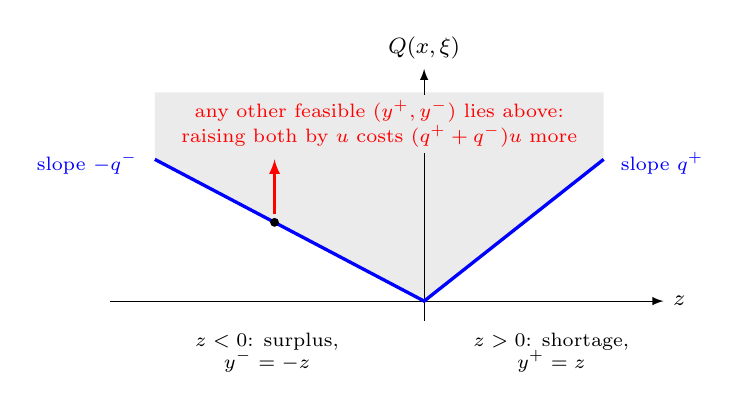
\begin{tikzpicture}[x=0.95cm,y=0.5cm,>=latex,font=\footnotesize]
  \fill[black!8] (-3.6,3.6) -- (0,0) -- (2.4,3.6) -- (2.4,5.3) -- (-3.6,5.3) -- cycle;
  \draw[->] (-4.2,0) -- (3.2,0) node[right]{$z$};
  \draw[->] (0,-0.5) -- (0,5.9) node[above]{$Q(x,\xi)$};
  \draw[blue,line width=1.2pt] (-3.6,3.6) -- (0,0) -- (2.4,3.6);
  \node[blue,left,font=\scriptsize]  at (-3.7,3.5) {slope $-q^-$};
  \node[blue,right,font=\scriptsize] at (2.5,3.5)  {slope $q^+$};
  \node[font=\scriptsize,align=center] at (-2.1,-1.3) {$z<0$: surplus,\\$y^-=-z$};
  \node[font=\scriptsize,align=center] at (1.7,-1.3)  {$z>0$: shortage,\\$y^+=z$};
  \fill (-2.0,2.0) circle (1.6pt);
  \draw[->,red,thick] (-2.0,2.2) -- (-2.0,3.6);
  \node[red,align=center,font=\scriptsize,fill=black!8,inner sep=2pt] at (-0.6,4.5)
     {any other feasible $(y^+,y^-)$ lies above:\\raising both by $u$ costs $(q^++q^-)u$ more};
\end{tikzpicture}
\end{center}

The V points upwards exactly when $q^+ + q^- \geq 0$; otherwise inflating $y^+$ and $y^-$ together is profitable and $Q(x,\xi) = -\infty$.

\end{frame}


\begin{frame}
\frametitle{Simple recourse (cont'd)}

\begin{itemize}
	\item 
Since the recourse is complete, it is feasible for any first-stage decision $x$.
\item
The following result establishes conditions to have a finite recourse (i.e. $| \calQ(x) | < \infty$).
\end{itemize}

\begin{theo}
Assume that the two-stage (linear) stochastic program is feasible and has a simple recourse, and that $\bsxi$ has finite second-order moments.
Then $\mathcal{Q}(x)$ is finite if and only if, for any component $i$, $\boldsymbol{q}_i^+ + \boldsymbol{q}_i^- \geq 0$ with probability one.
\end{theo}

\end{frame}

\begin{frame}
\frametitle{Simple recourse (cont'd)}

\begin{proof}
{\bf $(\Rightarrow)$} 
Assume by contradiction that $\mathcal{Q}$ is finite, but for some component $i$, $q_i^+(\xi(\omega)) + q_i^-(\xi(\omega)) < 0$ for $\omega \in \Omega_1$ with $P[\Omega_1] > 0$.
Then, for any feasible $x$, for all $\omega \in \Omega_1$ with $h_i(\xi(\omega))-T_i(\xi(\omega))x > 0$, define
$$
y_i^+(\xi(\omega)) = h_i(\xi(\omega)) - T_i(\xi(\omega))x + u,\  y_i^-(\xi(\omega)) = u.
$$
Therefore, 
$$
y_i^+(\xi(\omega)) - y_i^-(\xi(\omega)) = h_i(\xi(\omega)) - T_i(\xi(\omega))x,\ y_i^+ \geq 0,\ y_i^- \geq 0.
$$
%Therefore, $y_i^+ - y_i^-$ are feasible.
Moreover, %since $\mathcal{Q}(x)$ is finite, $Q(x, \xi(\omega))$ is feasible a.s.
%so, almost surely,
we can choose $y_j^+$ and $y_j^-$ feasible, $j \ne i$.

\end{proof}

\end{frame}

\begin{frame}
\frametitle{Simple recourse (cont'd)}

\begin{proof}
{\bf $(\Rightarrow)$} 

When $u \rightarrow \infty$, $Q(x, \xi(\omega)) \rightarrow -\infty$ since $q_i^+(\xi(\omega))y_i^+ + q_i^-(\xi(\omega))y_i^- \rightarrow -\infty$.

\mbox{}

A similar argument can be applied if $h_i(\xi(\omega))-T_i(\xi(\omega))x \leq 0$, by taking
$$
y_i^+(\xi(\omega)) = u,\ y_i^-(\xi(\omega)) = -h_i(\xi(\omega)) + T_i(\xi(\omega))x + u.
$$

\mbox{}

The two cases cover every $\omega \in \Omega_1$, so $Q(x,\xi(\omega)) = -\infty$ on a set of positive probability and $\mathcal{Q}(x) = -\infty$: the recourse is not finite.
\end{proof}

\end{frame}

\begin{frame}
\frametitle{Simple recourse (cont'd)}
\small
	
\begin{proof}

{\bf $(\Leftarrow)$}
Assume $\forall\, i$, $P[\boldsymbol{q}_i^+ + \boldsymbol{q}_i^- \geq 0] = 1$.
Write $z(\xi) = h(\xi)-T(\xi)x$. Any feasible $(y^+, y^-)$ satisfies $y^+-y^- = z(\xi)$, $y^+ \geq 0$, $y^- \geq 0$, so $y_i^- = y_i^+ - z_i(\xi)$ and its {\red objective value} is
\begin{align*}
\sum_{i=1}^{m} \left( q_i^+(\xi)y_i^+ + q_i^-(\xi)y_i^- \right)
&= \sum_{i=1}^{m} \left( q_i^+(\xi)y_i^+ + q_i^-(\xi)\left(y_i^+-z_i(\xi)\right) \right) \\
&= \sum_{i=1}^{m} \left( \left(q_i^+(\xi) + q_i^-(\xi)\right)y_i^+ - q_i^-(\xi)z_i(\xi) \right).
\end{align*}
This is the value at an arbitrary feasible point, not yet the optimal value $Q(x,\xi)$.

\end{proof}

\end{frame}

\begin{frame}
\frametitle{Simple recourse (cont'd)}
\small

\begin{proof}
{\bf $(\Leftarrow)$}

Almost surely $q_i^+(\xi) + q_i^-(\xi) \geq 0$, and $y_i^+ \geq 0$, so the first sum above is non-negative: {\red every} feasible point has an objective value at least $-q^-(\xi)^Tz(\xi)$. Taking the infimum,
$$
Q(x,\xi) \geq -q^-(\xi)^Tz(\xi) \quad \text{a.s.}
$$
The program is feasible and bounded below, so it admits an optimal solution.

\mbox{}

The objective being non-decreasing in each $y_i^+$, the infimum is attained at the smallest feasible $y_i^+$ (equivalently, at a basic solution, where at most one of $y_i^+$, $y_i^-$ is positive):
\begin{align*}
	y^+(\xi) &= \left(h(\xi)-T(\xi)x\right)^+, &
	y^-(\xi) &= \left(-h(\xi)+T(\xi)x\right)^+,
\end{align*}
where $a^+ = \max\{0, a\}$.

\end{proof}

\end{frame}

\begin{frame}
\frametitle{Simple recourse (cont'd)}

\begin{proof}
{\bf $(\Leftarrow)$}

At that optimum $Q(x,\xi) = \sum_{i=1}^m \left( q_i^+(\xi)z_i(\xi)^+ + q_i^-(\xi)(-z_i(\xi))^+ \right)$, hence
$|Q(x,\xi)| \leq \|q(\xi)\| \, \|z(\xi)\|$.

\mbox{}

{\red This is where the finite second-order moments are used}: $z(\xi) = h(\xi)-T(\xi)x$ is affine in $\xi$, so $\EE[\|z(\bsxi)\|^2] < \infty$, and Cauchy--Schwarz gives
$$
\EE\left[ \|q(\bsxi)\| \, \|z(\bsxi)\| \right] \leq
\left( \EE\left[\|q(\bsxi)\|^2\right] \right)^{1/2}
\left( \EE\left[\|z(\bsxi)\|^2\right] \right)^{1/2} < \infty.
$$
Therefore $|\calQ(x)| < \infty$: the recourse is finite, and in particular
$\calQ(x) \geq \EE_{\bsxi}\left[-q^-(\bsxi)^Tz(\bsxi)\right]$.
\end{proof}

\end{frame}

\begin{frame}
\frametitle{Exercise}
	
%(Birge and Louveaux, page 87)
Consider the second stage program
\[
Q(x, \xi) = \min_y \lbrace y \ |\ \xi y = 1-x, y \geq 0 \rbrace.
\]
We assume that $\bsxi$ follows a triangular distribution on $[0,1]$, with $P[\bsxi \leq u] = u^2$.
	
\mbox{}
	
{\blue (a)}
Is the recourse fixed? Why?
	
\mbox{}
	
The recourse is not fixed, as $W \equiv \bsxi$, and therefore, $W$ is random.
Moreover, as $\xi$ can take the value 0, the transformation
\[
y = 1/\xi - x/\xi,
\]
is not properly defined on $\Xi = [0,1]$; this also means that
\[
\text{pos}\,W =
\begin{cases}
\lbrace 0 \rbrace & \text{ if } \xi = 0; \\
\RR_+ & \text{ if } \xi \ne 0.
\end{cases}
\]
	
\end{frame}

\begin{frame}
\frametitle{Exercise (cont'd)}
	
{\blue (b)} Express $K_2(\xi)$ for all $\xi$ in $[0,1]$.
	
\mbox{}
	
We have to consider two cases: $\xi = 0$ or $\xi \in (0,1]$.
	
\mbox{}
	
{\red 1. $\xi \in (0,1]$} In this case, as $y, \xi \geq 0$, $1-x$ has to be non-negative in order to have a well-defined problem:
\[
K_2(\xi) = \lbrace x\,|\, x \leq 1 \rbrace.
\]

The value and optimal solutions are
\[
Q(x,\xi) = (1-x)/\xi,\quad y^*= (1-x)/\xi.
\]
	
{\red 2. $\xi=0$} There exists no $y$ such that $0.y = 1-x$, except if $x = 1$, so
\[
K_2(0) = \lbrace 1 \rbrace.
\]
	
\end{frame}

\begin{frame}
\frametitle{Exercise (cont'd)}
	
{\blue (c)} Express $K_2$, $K_2^P$ and $\mathcal{Q}$.
	
\mbox{}
	
From the previous point, we have
\[
K_2^P = \lbrace x \,|\, x \leq 1 \rbrace \cap \lbrace 1 \rbrace =
\lbrace 1 \rbrace.
\]
We also have, as $P[\xi = 0] = 0$,
\[
\mathcal{Q}(x) = \int_0^1 \frac{1-x}{\xi} 2\xi d\xi = 2(1-x), \forall
x \leq 1.
\]
Consequently $K_2^P \subset K_2 = \lbrace x \leq 1 \rbrace$.

The difference comes from the fact that a point is not in $K_2^P$ as soon as it is not feasible for a given value of $\xi$, but $K_2$ does not consider infeasible situations that occur with a null probability.
	With a {\red fixed} recourse --- not the case here --- and finite second-order moments, we would have had $K_2 = K_2^P$.
	
\end{frame}

\begin{frame}
\frametitle{Convexity of $v(\xi, \cdot)$}

Let $y^*_1$ and $y^*_2$ be two optimal solutions of $v(\xi, z)$, associated to $z = z_1$ and $z = z_2$, respectively.
Then, the convex combination $y_{\alpha} \overset{\mathrm{def}}{=} \alpha y_1^*+(1-\alpha)y_2^*$, $\alpha \in [0,1]$, is feasible with respect to $z_{\alpha} = \alpha z_1 + (1-\alpha) z_2$, as $\alpha y_1^*+(1-\alpha)y_2^* \geq 0$, and
$$
W(\alpha y_1^*+(1-\alpha)y_2^*)
= \alpha W y_1^* + (1-\alpha) W y_2^*
= \alpha z_1 + (1-\alpha) z_2 = z_{\alpha}.
$$
Since $y_{\alpha}$ is feasible for $z_{\alpha}$, the definition of $v$ as an infimum gives directly
\begin{align*}
v(\xi, z_{\alpha}) & \leq q(\xi)^T y_{\alpha} = q(\xi)^T(\alpha y_1^*+(1-\alpha)y_2^*) \\
& = \alpha q(\xi)^T y_1^*+(1-\alpha)q(\xi)^Ty_2^* \\
& = \alpha v(\xi, z_1) + (1-\alpha) v(\xi, z_2).
\end{align*}
In other words, $v$ is a convex function w.r.t. $z \in \RR^m$.
No optimal solution has to be assumed at $z_{\alpha}$: only feasibility of $y_{\alpha}$ is used.

%\mbox{}

%We also have the well-known property
%\begin{theo}
%If $f_1(x)$, $f_2(x)$,\ldots,$f_q(x)$ is an arbitrary collection of convex functions, then $M(x) = \max \lbrace f_1(x), f_2(x),\ldots,f_q(x) \rbrace$ is also a convex function.
%\end{theo}
\end{frame}

\begin{frame}
\frametitle{Convexity of second-stage function}

$Q(x,\xi)$ is the value function of a linear program, seen as a function of its right-hand side $h(\xi)-T(\xi)x$ and of its costs: the properties below are those recalled in the linear programming background notes.

We have the following result (Birge and Louveaux, Chapter~3, Theorem~5).
\begin{theo}
For a stochastic program with fixed recourse, $Q(x,\xi)$ is
\begin{enumerate}[(a)]
\item
a piecewise-linear convex function in $(h,T)$,
\item
a piecewise-linear concave function in $q$,
\item
a piecewise-linear convex function in $x$, for all $x$ in $K = K_1 \cap K_2$.
\end{enumerate}
\end{theo}

(a) and (c) follow from the convexity of $v(\xi, \cdot)$ just established, composed with the affine map $x \mapsto h(\xi)-T(\xi)x$; (b) is the concavity of the value function in the costs; the piecewise linearity comes from the finite number of optimal bases.

\end{frame}

\begin{frame}
\frametitle{Convexity of the recourse}

$\mathcal{Q}(x) = \EE_{\bsxi} [Q(x,\bsxi)]$. Suppose for now that $\bsxi$ has a finite support,
$\Xi = \lbrace \xi_1, \xi_2,\ldots, \xi_S \rbrace$, so that
$\mathcal{Q}(x) = \sum_{s = 1}^{S} P[\bsxi = \xi_s] Q(x,\xi_s)$.

\begin{theo}
A non-negative combination of convex functions is convex: if $f_1,\ldots,f_K$ are convex and $\alpha_1,\ldots,\alpha_K \geq 0$, then $\sum_{k=1}^K \alpha_k f_k$ is convex.
\end{theo}

$\mathcal{Q}(x)$ is therefore a convex function w.r.t. $x$.

\mbox{}

What is happening in the continuous case?
The same argument applies verbatim to any measure: if $g(\cdot, t)$ is convex for every $t$, then $x \mapsto \int g(x,t)\,d\mu(t)$ is convex, an integral being a limit of non-negative combinations. Since
\[
\mathcal{Q}(x) = \int_{\Xi} Q(x,t) dF(t),
\]
{\red $\mathcal{Q}(x)$ is convex}.

\end{frame}

\begin{frame}
\frametitle{An example\ldots}

Consider the second-stage function $Q(x,\xi)$ defined as:
\begin{align*}
\min y^++y^- \mbox{ s.t. } y^+-y^- = \xi - x,\ y^+ \geq 0,\ y^- \geq 0.
\end{align*}
In other words:
\[
y = \begin{pmatrix} y^+ \\ y^- \end{pmatrix} \quad q = \begin{pmatrix}
    1 \\ 1 \end{pmatrix}, W = \begin{pmatrix} 1 & -1 \end{pmatrix}
  \quad h(\xi) = \xi \quad T(\xi) = 1.
\]

\mbox{}

Relying on the fundamental theorem of linear programming, we are looking for an optimal basic solution, implying that $y^+ = 0$ or $y^- = 0$.

\end{frame}

\begin{frame}
\frametitle{An example\ldots (cont'd)}

We immediately see that
$$
y^+ = \begin{cases}
	\xi - x & \text{ if } \xi - x \geq 0, \\
	0 & \text{otherwise,}
\end{cases}
$$
and
$$
y^- = \begin{cases}
	-\xi + x & \text{ if } \xi - x < 0, \\
	0 & \text{otherwise.}
\end{cases}
$$

\end{frame}

\begin{frame}
\frametitle{An example: the dual and the optimality conditions}

Dual, with the slacks $s_1$, $s_2$ made explicit:
\begin{align*}
\max_{\pi}\ & (\xi-x)\pi \qquad \text{s.t. } \pi \leq 1,\ -\pi \leq 1 \\
\Longleftrightarrow\ \max_{\pi}\ & (\xi-x)\pi \qquad \text{s.t. }
\pi + s_1 = 1,\ -\pi + s_2 = 1,\ s_1, s_2 \geq 0.
\end{align*}

The recourse is simple, and the primal-dual/KKT conditions of the background notes give
\begin{align*}
\begin{pmatrix} 1 \\ 1 \end{pmatrix} & = \begin{pmatrix} 1 \\
  -1 \end{pmatrix} \pi + \begin{pmatrix} s_1 \\ s_2 \end{pmatrix}
  & \text{(dual feasibility)} \\
y^+ - y^- & = \xi - x & \text{(primal feasibility)} \\
y^+ &\geq 0,\  y^- \geq 0,\ s_1 \geq 0,\ s_2 \geq 0 \\
s_1y^+ & = 0,\ s_2y^- = 0 & \text{(complementary slackness)}.
\end{align*}

\end{frame}

\begin{frame}
\frametitle{An example (cont'd)}

\begin{itemize}
\item
The first condition implies that we cannot have
$s_1 = s_2 = 0$.
\item
From the complementarity conditions, we have that $y^+ = 0$ or $y^-
= 0$.
\item
We have to consider two cases:
\begin{itemize}
\item
$x \leq \xi$: in this situation, we have
\[
y^+ = \xi -x,\quad y^- = 0.
\]
\item
$x \geq \xi$: then,
\[
y^- = x-\xi,\quad y^+ = 0.
\]
\end{itemize}
\item
Consequently,
\[
Q(x,\xi) = \begin{cases} \xi-x & \text{ if } x \leq \xi, \\
	x - \xi & \text{ if } x \geq \xi, \end{cases}
\]
that is, $Q(x,\xi) = |\xi - x|$.
\end{itemize}

\end{frame}

\begin{frame}
\frametitle{Graphically?}

Assume that $\bsxi$ can take the realizations $1$, $2$, $4$.

\begin{center}
\begin{minipage}{0.9\textwidth}

\includegraphics[width=0.85\textwidth]{recourse_1.pdf}
\end{minipage}
\end{center}

\end{frame}

\begin{frame}
\frametitle{Graphically (cont'd)}

\begin{center}
\begin{minipage}{0.9\textwidth}

\includegraphics[width=0.85\textwidth]{recourse_2.pdf}
\end{minipage}
\end{center}

\end{frame}

\begin{frame}
\frametitle{Graphically (cont'd)}

\begin{center}
\begin{minipage}{0.9\textwidth}

\includegraphics[width=0.85\textwidth]{recourse_4.pdf}
\end{minipage}
\end{center}

\end{frame}

\begin{frame}
\frametitle{$\mathcal{Q}(x)$}

What about $\mathcal{Q}(x)$?

\mbox{}

Assume that the three realizations have the same probability.

\mbox{}

We have to consider 4 cases:
\begin{enumerate}
\item
$x \leq 1$: $\mathcal{Q}(x) = 7/3 - x$;
\item
$1 \leq x \leq 2$: $\mathcal{Q}(x) = 5/3-x/3$;
\item
$2 \leq x \leq 4$: $\mathcal{Q}(x) = x/3+1/3$;
\item
$4 \leq x$: $\mathcal{Q}(x) = x-7/3$;
\end{enumerate}

\end{frame}

\begin{frame}
\frametitle{Where the kinks come from}

\begin{center}
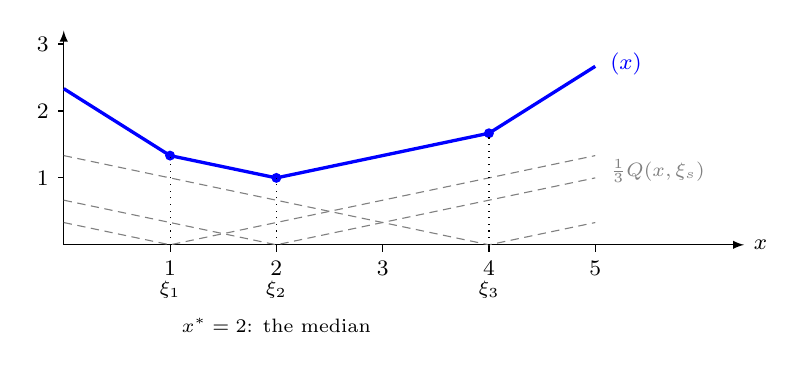
\begin{tikzpicture}[x=1.35cm,y=0.85cm,>=latex,font=\footnotesize]
  \draw[->] (0,0) -- (6.4,0) node[right]{$x$};
  \draw[->] (0,0) -- (0,3.2);
  \foreach \i in {1,...,5} \draw (\i,0) -- (\i,-0.1) node[below]{$\i$};
  \foreach \j in {1,2,3} \draw (0,\j) -- (-0.05,\j) node[left]{$\j$};
  % the three scaled scenario costs
  \draw[gray,densely dashed] (0,0.333) -- (1,0) -- (5,1.333);
  \draw[gray,densely dashed] (0,0.667) -- (2,0) -- (5,1.0);
  \draw[gray,densely dashed] (0,1.333) -- (4,0) -- (5,0.333);
  % the expected recourse
  \draw[blue,line width=1.2pt] (0,2.333) -- (1,1.333) -- (2,1) -- (4,1.667) -- (5,2.667);
  \foreach \p/\q in {1/1.333, 2/1, 4/1.667} {
     \fill[blue] (\p,\q) circle (1.8pt);
     \draw[dotted] (\p,0) -- (\p,\q);
  }
  \node[below,font=\scriptsize] at (1,-0.4) {$\xi_1$};
  \node[below,font=\scriptsize] at (2,-0.4) {$\xi_2$};
  \node[below,font=\scriptsize] at (4,-0.4) {$\xi_3$};
  \node[blue,right] at (5.05,2.7) {$\calQ(x)$};
  \node[gray,right,font=\scriptsize] at (5.05,1.1) {$\frac13 Q(x,\xi_s)$};
  \node[below,font=\scriptsize] at (2,-0.95) {$x^\ast=2$: the median};
\end{tikzpicture}
\end{center}

Each scenario contributes one kink, at its own realization; $\calQ$ is their non-negative weighted sum, hence convex and piecewise linear, and its minimizer is here the median of the scenarios.

\end{frame}


\begin{frame}
\frametitle{Properties of $\mathcal{Q}(x)$}

$\mathcal{Q}(x)$ is convex; it is moreover piecewise linear {\red when the support of $\bsxi$ is finite}, where it is a non-negative weighted sum of the $Q(\cdot,\xi_s)$, each of which has just been shown to be convex and piecewise linear.
On a continuous support the piecewise linearity is lost, as the smoothing frame below shows.
The general statement is the following.

\begin{theo}
For a stochastic program with fixed recourse where $\bsxi$ has finite second-order moments,
\begin{enumerate}[(a)]
\item
$\mathcal{Q}(x)$ is convex, and finite and Lipschitz continuous on $K_2$;
\item
when $\bsxi$ has a finite support, $\mathcal{Q}(x)$ is piecewise linear.
\end{enumerate}
\end{theo}

Reminder: a function $f$ is Lipschitz if there exists some $M < \infty$ such that for all $x$, $y$,
\[
|f(x)-f(y)| \leq M \| x-y \|.
\]

\end{frame}

\begin{frame}
\frametitle{Differentiability of the recourse}

Is $\mathcal{Q}(x)$ also differentiable?

\mbox{}

The recourse function is partially differentiable with respect to $x_j$ at $(\hat{x}, \hat{\xi})$ if the directional derivative exists for the direction $e_j$.
In other words, there exists a function $\frac{\partial Q(x,\xi)}{\partial x_j}$ such that
\[
\frac{Q(\hat{x}+he_j,\hat{\xi}) - Q(\hat{x},\hat{\xi})}{h} =
\frac{\partial Q(\hat{x},\hat{\xi})}{\partial x_j} + \frac{\rho_j (\hat{x},
  \hat{\xi}; h)}{h},
\]
with
\[
\frac{\rho_j (\hat{x}, \hat{\xi}; h)}{h} \rightarrow 0, \mbox{ as } h\rightarrow 0.
\]

\mbox{}

We will assume from now that $\nabla_x Q(x, \xi) = \left( \frac{\partial
  Q(x,\xi)}{\partial x_1},\ldots, \frac{\partial
  Q(x,\xi)}{\partial x_n} \right)$ exists.

\end{frame}

\begin{frame}
\frametitle{Differentiability of the recourse (cont'd)}
\small

What about the differentiability of $\mathcal{Q}(x)$?

\begin{align*}
\frac{\mathcal{Q}(\hat{x}+he_j) -
  \mathcal{Q}(\hat{x})}{h} &=
\int_{\Xi}
\frac{Q(\hat{x}+he_j,\xi) - Q(\hat{x},\xi)}{h} dP \\
&= \int_{\Xi \backslash N_{\delta}} \frac{\partial
  Q(\hat{x},\xi)}{\partial x_j} dP+ \int_{\Xi \backslash N_{\delta}}
\frac{\rho_j (\hat{x}, \xi; h)}{h} dP,
\end{align*}
where $N_{\delta}$ is measurable and $P[N_{\delta}] = 0$.
Therefore, we have
\begin{theo}
If $Q(x,\xi)$ is partially differentiable almost everywhere, if its partial derivative 
$\frac{\partial Q(\hat{x},\xi)}{\partial x_j}$ is integrable and if the residual satisfies
$(1/h) \int_{\Xi \backslash N_{\delta}} \rho_j (\hat{x}, \xi; h) dP \overset{h \rightarrow 0}{\rightarrow } 0$, then $\frac{\partial \mathcal{Q}(\hat{x})}{\partial x_j}$ exists and
\[
 \frac{\partial \mathcal{Q}(\hat{x})}{\partial x_j} =
 \int_{\Xi} \frac{\partial Q(\hat{x},\xi)}{\partial x_j} dP.
\]
\end{theo}

\end{frame}

\begin{frame}
\frametitle{Differentiability of the recourse: discrete case}

The residual condition $(1/h) \int_{\Xi
  \backslash N_{\delta}} \rho_j (\hat{x}, \xi; h) dP \overset{h
  \rightarrow 0}{\rightarrow } 0$ {\red cannot hold everywhere} here.

\mbox{}

Indeed, in the linear framework with fixed recourse, and for vectors $\bsxi$ with finite second-order moments, we have seen that $\mathcal{Q}(x)$ is piecewise linear when $\bsxi$ has a finite support.
It is therefore differentiable {\red except} at its finitely many kinks --- and it is precisely at a kink that the residual condition fails.
There, we will have to work with subgradients.

\end{frame}

\begin{frame}
\frametitle{Differentiability of the recourse: continuous case}

If $\bsxi$ is continuous, $\mathcal{Q}(x)$ is obtained as an integral over the $Q(x,\xi)$'s, that are not differentiable as they are piecewise linear given $\xi$.
However, it is $x$ that has to be fixed, not $\xi$.
It is possible to show that (the proof is quite technical)

\mbox{}

\begin{theo}
For a stochastic program with fixed recourse where $\bsxi$ has finite second-order moments, if $\bsxi$ has an absolutely continuous distribution, then $\mathcal{Q}(x)$ is differentiable on the interior of $K_2$.
\end{theo}

\mbox{}

Intuitively, the function $\mathcal{Q}(x)$ is ``smoothed'' by the superposition of an infinite number of functions $Q(x,\xi)$.

\end{frame}

\begin{frame}
\frametitle{Smoothing by superposition}

Same family $Q(x,\xi) = |x-\xi|$, with $\bsxi$ spread more and more finely over $[1,4]$.

\begin{center}
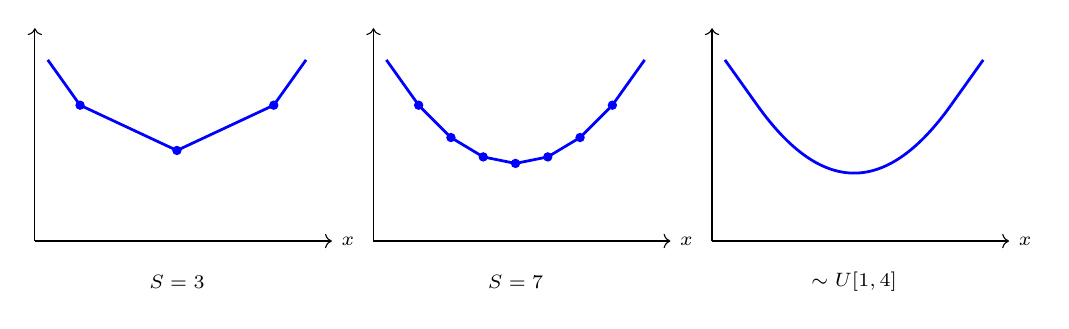
\begin{tikzpicture}[x=0.82cm,y=1.15cm,font=\footnotesize]
 \foreach \dx/\cap in {0/{$S=3$}, 4.3/{$S=7$}, 8.6/{$\bsxi \sim U[1,4]$}} {
  \begin{scope}[xshift=\dx cm]
    \draw[->] (0.3,0) -- (4.9,0) node[right,font=\scriptsize]{$x$};
    \draw[->] (0.3,0) -- (0.3,2.35);
    \node[font=\scriptsize] at (2.5,-0.45) {\cap};
  \end{scope}}
  % S = 3: realizations 1, 2.5, 4
  \draw[blue,line width=1pt] (0.5,2.0) -- (1,1.5) -- (2.5,1) -- (4,1.5) -- (4.5,2.0);
  \foreach \p/\q in {1/1.5, 2.5/1, 4/1.5} \fill[blue] (\p,\q) circle (1.7pt);
  % S = 7: realizations 1, 1.5, ..., 4
  \begin{scope}[xshift=4.3cm]
    \draw[blue,line width=1pt] (0.5,2.0) -- (1,1.5) -- (1.5,1.143) -- (2,0.929)
       -- (2.5,0.857) -- (3,0.929) -- (3.5,1.143) -- (4,1.5) -- (4.5,2.0);
    \foreach \p/\q in {1/1.5, 1.5/1.143, 2/0.929, 2.5/0.857, 3/0.929, 3.5/1.143, 4/1.5}
       \fill[blue] (\p,\q) circle (1.7pt);
  \end{scope}
  % continuous
  \begin{scope}[xshift=8.6cm]
    \draw[blue,line width=1pt] (0.5,2.0) -- (1,1.5);
    \draw[blue,line width=1pt] plot[domain=1:4,samples=40,smooth]
        (\x,{((\x-1)*(\x-1)+(4-\x)*(4-\x))/6});
    \draw[blue,line width=1pt] (4,1.5) -- (4.5,2.0);
  \end{scope}
\end{tikzpicture}
\end{center}

\smallskip

The tails are identical; only the middle changes. With finitely many scenarios $\calQ$ keeps one kink per scenario; in the limit the kinks are averaged away and $\calQ$ becomes differentiable on the interior of $K_2$.

\end{frame}


\begin{frame}
\frametitle{The value of information}

Uncertainty has a cost.
Two natural questions:
\begin{itemize}
\item
how much would we gain if the uncertainty could be removed {\red before} deciding?
\item
how much do we lose if we simply replace $\bsxi$ by its mean?
\end{itemize}

\mbox{}

Write the total cost attached to a first-stage decision $x$ and a realization $\xi$ as
\[
z(x,\xi) \overset{\mathrm{def}}{=} c^Tx + Q(x,\xi).
\]
The problem studied so far is the {\red recourse problem}
\[
\RP \overset{\mathrm{def}}{=} \min_{x \in K_1 \cap K_2} \EE_{\bsxi}[z(x,\bsxi)] = \min_{x \in K_1 \cap K_2} \lbrace c^Tx + \calQ(x) \rbrace,
\]
and we denote by $x^*$ one of its optimal solutions.

\end{frame}

\begin{frame}
\frametitle{Wait-and-see}

If $\bsxi$ could be observed {\red before} deciding on $x$, we would solve one deterministic program per realization, and the expected cost would be the {\red wait-and-see} value
\[
\WS \overset{\mathrm{def}}{=} \EE_{\bsxi} \left[ \min_{x \in K_1 \cap K_2(\bsxi)} z(x,\bsxi) \right].
\]
Note the position of the expectation: in $\RP$, a {\blue single} $x$ has to serve all the realizations, while in $\WS$ the decision may depend on $\xi$.

\mbox{}

The {\red expected value of perfect information} is
\[
\EVPI \overset{\mathrm{def}}{=} \RP - \WS.
\]
It measures the maximum price a decision maker should be ready to pay for a perfect forecast of $\bsxi$.

\end{frame}

\begin{frame}
\frametitle{$\EVPI \geq 0$}

\begin{theo}
$\WS \leq \RP$, and therefore $\EVPI \geq 0$.
\end{theo}

\begin{proof}
Let $x$ be any feasible first-stage decision, i.e. $x \in K_1 \cap K_2$.
For almost every realization $\xi$, $x$ is feasible for the second stage, so
\[
\min_{x' \in K_1 \cap K_2(\xi)} z(x',\xi) \leq z(x,\xi).
\]
Taking the expectation preserves the inequality:
\[
\WS \leq \EE_{\bsxi}[z(x,\bsxi)].
\]
The left-hand side does not depend on $x$: minimizing the right-hand side over all feasible $x$ gives $\WS \leq \RP$.
\end{proof}

\end{frame}

\begin{frame}
\frametitle{The expected value problem}

A cheaper alternative is to ignore the randomness and to solve a single deterministic program built on $\overline{\xi} \overset{\mathrm{def}}{=} \EE[\bsxi]$: the {\red expected value (EV) problem}
\[
\EV \overset{\mathrm{def}}{=} \min_{x \in K_1 \cap K_2(\overline{\xi})} z(x,\overline{\xi}),
\]
whose optimal solution is denoted $\overline{x}(\overline{\xi})$.

\mbox{}

$\overline{x}(\overline{\xi})$ is a legitimate first-stage decision, but it has been computed while ignoring the variability of $\bsxi$.
Its true expected cost is the {\red expected result of using the EV solution}
\[
\EEV \overset{\mathrm{def}}{=} \EE_{\bsxi}\left[ z(\overline{x}(\overline{\xi}),\bsxi) \right],
\]
and the {\red value of the stochastic solution} is
\[
\VSS \overset{\mathrm{def}}{=} \EEV - \RP.
\]

\end{frame}

\begin{frame}
\frametitle{$\VSS \geq 0$}

\begin{theo}
$\RP \leq \EEV$, and therefore $\VSS \geq 0$.
\end{theo}

\begin{proof}
By construction $\overline{x}(\overline{\xi}) \in K_1$; if it does not belong to $K_2$, then $\calQ(\overline{x}(\overline{\xi})) = +\infty$, so $\EEV = +\infty$ and the result is immediate.
Otherwise, $\overline{x}(\overline{\xi})$ is a particular feasible point of the recourse problem, so
\[
\RP = \min_{x \in K_1 \cap K_2} \EE_{\bsxi}[z(x,\bsxi)] \leq \EE_{\bsxi}\left[z(\overline{x}(\overline{\xi}),\bsxi)\right] = \EEV.
\]
\end{proof}

$\VSS$ measures what is gained by modelling the uncertainty explicitly, rather than replacing it by its mean.

\end{frame}

\begin{frame}
\frametitle{A chain of bounds}

\begin{theo}
If only the right-hand side $h(\bsxi)$ is random, $W$, $T$ and $q$ being fixed, and $h$ depends affinely on $\xi$, then $\EV \leq \WS$.
\end{theo}
\begin{proof}
Set $\psi(\xi) \overset{\mathrm{def}}{=} \min_{x \in K_1 \cap K_2(\xi)} z(x,\xi)$.
As $W$, $T$ and $q$ are fixed, $\psi(\xi)$ is the optimal value of a linear program whose only varying data is the right-hand side; such a value function is convex (background notes), here in $h(\xi)$, hence in $\xi$.
Jensen's inequality then gives
\[
\EV = \psi(\EE[\bsxi]) \leq \EE_{\bsxi}[\psi(\bsxi)] = \WS.
\]
\end{proof}
If $T$ is random, $\psi$ is no longer an optimal value with respect to the right-hand side only, and the argument does not apply.
Collecting the results:
\[
\EV \leq \WS \leq \RP \leq \EEV.
\]
\end{frame}

\begin{frame}
\frametitle{The four values on one axis}

\begin{center}
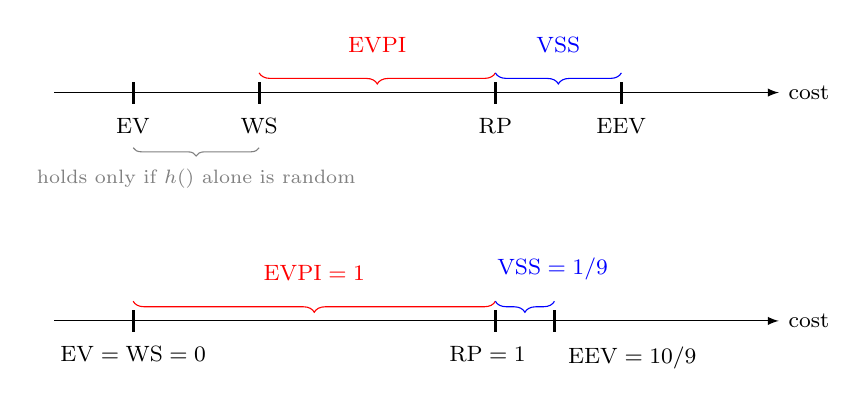
\begin{tikzpicture}[x=1cm,y=1cm,>=latex,font=\footnotesize]
  \draw[->] (0,0) -- (9.2,0) node[right]{cost};
  \foreach \p/\l in {1.0/\EV, 2.6/\WS, 5.6/\RP, 7.2/\EEV} {
    \draw[line width=1pt] (\p,-0.14) -- (\p,0.14);
    \node[below] at (\p,-0.2) {$\l$};}
  \draw[decorate,decoration={brace,amplitude=4pt},red]
     (5.6,0.25) -- (2.6,0.25) node[midway,above=4pt,red]{$\EVPI$};
  \draw[decorate,decoration={brace,amplitude=4pt},blue]
     (7.2,0.25) -- (5.6,0.25) node[midway,above=4pt,blue]{$\VSS$};
  \draw[decorate,decoration={brace,amplitude=3pt,mirror},gray]
     (1.0,-0.7) -- (2.6,-0.7);
  \node[below,font=\scriptsize,align=center,gray] at (1.8,-0.85)
     {holds only if $h(\bsxi)$ alone is random};
  % --- the numerical example
  \begin{scope}[yshift=-2.9cm]
    \draw[->] (0,0) -- (9.2,0) node[right]{cost};
    \foreach \p in {1.0, 5.6, 6.35} \draw[line width=1pt] (\p,-0.14) -- (\p,0.14);
    \node[below] at (1.0,-0.2) {$\EV=\WS=0$};
    \node[below] at (5.5,-0.2) {$\RP=1$};
    \node[below right] at (6.4,-0.2) {$\EEV=10/9$};
    \draw[decorate,decoration={brace,amplitude=4pt},red]
       (5.6,0.25) -- (1.0,0.25) node[midway,above=4pt,red]{$\EVPI=1$};
    \draw[decorate,decoration={brace,amplitude=4pt},blue]
       (6.35,0.25) -- (5.6,0.25) node[midway,above=4pt,blue,xshift=10pt]{$\VSS=1/9$};
  \end{scope}
\end{tikzpicture}
\end{center}

\end{frame}


\begin{frame}
\frametitle{Example}

Take again $Q(x,\xi) = |x-\xi|$ with $\bsxi$ uniform over $\lbrace 1, 2, 4 \rbrace$, and assume that the first stage has no direct cost ($c = 0$), so that $z(x,\xi) = Q(x,\xi)$ and, as computed previously,
\[
\calQ(x) = \begin{cases}
7/3 - x & \text{ if } x \leq 1, \\
5/3 - x/3 & \text{ if } 1 \leq x \leq 2, \\
x/3 + 1/3 & \text{ if } 2 \leq x \leq 4, \\
x - 7/3 & \text{ if } x \geq 4.
\end{cases}
\]
\begin{itemize}
\item
{\blue $\RP$}: the slope of $\calQ$ changes sign at $x^* = 2$, the median of the scenarios, so
$
\RP = \calQ(2) = 1.
$
\item
{\blue $\WS$}: for each realization, $\min_x |x-\xi| = 0$, attained at $x = \xi$. Hence
$
\WS = 0$, and $\EVPI = 1.
$
\end{itemize}

\end{frame}

\begin{frame}
\frametitle{Example (cont'd)}

\begin{itemize}
\item
{\blue $\EV$}: $\overline{\xi} = \EE[\bsxi] = (1+2+4)/3 = 7/3$, and $\min_x |x-7/3| = 0$ at $\overline{x}(\overline{\xi}) = 7/3$, so $\EV = 0$.
\item
{\blue $\EEV$}: the mean-value decision is now confronted with the three scenarios,
\[
\EEV = \calQ(7/3) = \frac{1}{3}\left( \frac{4}{3}+\frac{1}{3}+\frac{5}{3} \right) = \frac{10}{9},
\]
so that
\[
\VSS = \EEV - \RP = \frac{10}{9}-1 = \frac{1}{9}.
\]
\end{itemize}
We indeed have $\EV = 0 \leq \WS = 0 \leq \RP = 1 \leq \EEV = 10/9$.
Here perfect information is worth much more than a better use of the distribution: $\EVPI = 1 \gg \VSS = 1/9$.

\end{frame}

\begin{frame}
\frametitle{Remarks}

\begin{itemize}
\item
There is no general ordering between $\EVPI$ and $\VSS$: either one can be the larger.
\item
$\EEV$, and therefore $\VSS$, can be infinite: the mean-value decision $\overline{x}(\overline{\xi})$ may be infeasible for some scenarios.
A relatively complete recourse rules this out.
\item
The definitions above are written for a minimization problem.
For a maximization, $\EVPI = \WS - \RP$ and $\VSS = \RP - \EEV$.
For the farmer problem of the first chapter, $\WS = \$115406$, $\RP = \$108390$ and $\EEV = \$107240$, so $\EVPI = \$7016$ and $\VSS = \$1150$.
\item
Computing $\WS$ requires one deterministic program per realization, and $\EEV$ requires the recourse cost of $\overline{x}(\overline{\xi})$ over the whole support: both are out of reach as soon as the support is large, and are then estimated by sampling.
\end{itemize}

See Birge and Louveaux, Chapter~4.

\end{frame}

\begin{frame}
\frametitle{Two-stage non-linear problems}
\small

Now consider the general program
\[
\min_{x \in X} \EE_{\bsxi} [ f_0(x, \bsxi) ] = \min_{x \in X}
\EE_{\bsxi} [g_0(x,\bsxi) + Q(x, \bsxi)].
\]

\begin{theo}
If $g_0(\cdot,\xi)$ and $ Q(\cdot, \xi)$ are convex with respect to $x$, $\forall\ \xi \in \Xi$, and if $X$ is a convex set, the aforementioned program is convex.
\end{theo}
\begin{proof}
For $x_1$, $x_2 \in X$, $\lambda \in (0,1)$ and $x_{\lambda} = \lambda x_1 + (1-\lambda) x_2$, convexity in $x$ gives
\begin{multline*}
g_0(x_{\lambda}, \xi) + Q(x_{\lambda}, \xi) \\
\leq \lambda (g_0(x_1, \xi) + Q(x_1,
\xi)) + (1-\lambda)(g_0(x_2, \xi) + Q(x_2, \xi)).
\end{multline*}
Expectation preserves it, so the objective is convex; $X$ being convex, so is the program.
\end{proof}

\end{frame}

\begin{frame}
\frametitle{In a more standard form}

Inspired from Birge and Louveaux, Section~3.4.

\mbox{}

We consider the problem
\begin{align*}
\inf z &= f^1(x) + \mathcal{Q}(x), \\
\mbox{s.t. } & g_i^1(x) \leq 0,\ i = 1,\ldots,\overline{m}_1, \\
& g_i^1(x) = 0,\ i = \overline{m}_1+1,\ldots,m_1,
\end{align*}
where $\mathcal{Q}(x) = \EE_{\omega}[Q(x,\omega)]$ and
\begin{align*}
Q(x,\omega) &= \inf f^2(y(\omega), \omega), \\
\mbox{s.t. } & t_i^2(x, \omega) + g_i^2(y(\omega), \omega) \leq 0,\ i
= 1,\ldots,\overline{m}_2,\\
& t_i^2(x, \omega) + g_i^2(y(\omega), \omega) = 0,\ i =
\overline{m}_2+1,\ldots,m_2,
\end{align*}

\mbox{}

We say that the recourse is additive (why?).

\end{frame}

\begin{frame}
\frametitle{In a more standard form (cont'd)}

The functions $f^2(\cdot, \omega)$, $t_i^2(\cdot, \omega)$, and $g_i^2(\cdot, \omega)$ are continuous for any given $\omega$, and measurable w.r.t. $\omega$ for any given first argument.
This allows one to prove that $Q(x,\omega)$ is measurable, and therefore that $\mathcal{Q}(x)$ is well defined.

\mbox{}

Reintroduce $K_1$, $K_2(\omega)$ and $K_2^s$.

\begin{align*}
K_1 & = \lbrace x \ |\ g_i^1(x) \leq 0,\ i =
1,\ldots,\overline{m}_1, \\
& \quad \qquad g_i^1(x) = 0,\ i = \overline{m}_1+1,\ldots,m_1 \rbrace, \\
K_2(\omega) & = \lbrace x \ |\ \exists\, y(\omega) \mbox{ s.t. }
 t_i^2(x, \omega) + g_i^2(y(\omega), \omega) \leq 0,\ i
= 1,\ldots,\overline{m}_2,\\
& \quad \qquad t_i^2(x, \omega) + g_i^2(y(\omega), \omega) = 0, \ i =
\overline{m}_2+1,\ldots,m_2 \rbrace, \\
K_2^s & = \lbrace x \ |\ \mathcal{Q}(x) < \infty \rbrace.
\end{align*}

\end{frame}

\begin{frame}
\frametitle{Remarks}

The formulation is not yet totally general.
We will consider more general forms when we discuss sampling techniques.

\mbox{}

Here, there is no longer a fixed recourse, but the first-stage decision $x$ acts separately in the constraints.
Goal: extend the previous results.

\mbox{}

Questions: convexity, differentiability, optimality.
We should also consider the concept of lower semi-continuity.

\end{frame}

\end{document}